\documentclass{article}
\usepackage{amsmath}  % For math symbols
\usepackage{array}
\usepackage{graphicx} % Required for inserting images
\usepackage{lipsum}   % For dummy text, you can remove this if unnecessary
\usepackage{hyperref} % Include the hyperref package
\usepackage{subfigure}


\title{

\includegraphics[width=0.5\textwidth]{ist-logo.jpg}\\[1ex] % Image at the top, adjust width if needed
Machine Learning Report \\ 
\large Homework IV - Clustering and PCA
}
\author{ist1114964 - Axel Carapinha \\ ist1106565 - Martim Gordino}
\date{\today}

\begin{document}

\maketitle
\tableofcontents
\newpage

\section{Clustering}
\subsection{Exercise a)}

Firstly, by analysing the given information, we already know that:

\[
x_1 = \begin{pmatrix} 1 \\ 1 \end{pmatrix} , x_2 = \begin{pmatrix} -1 \\ -1 \end{pmatrix} , x_3 = \begin{pmatrix} 0.5 \\ 0.55 \end{pmatrix}
\]

\[
P(x \mid C = 1) = N\left(\mu^1 = \begin{pmatrix} 1 \\ 1 \end{pmatrix}, \quad \Sigma_1 = \begin{pmatrix} 1 & 0 \\ 0 & 1 \end{pmatrix}\right)
\]
\[
P(x \mid C = 2) = N\left(\mu^2 = \begin{pmatrix} -1 \\ -1 \end{pmatrix}, \quad \Sigma_2 = \begin{pmatrix} 1 & 0 \\ 0 & 1 \end{pmatrix}\right)
\]

We also know the prior probabilities of C:
\[
P(C = 1) = 0.6
\]
\[
P(C = 2) = 0.4
\]
\newline
Now we can get to the second step, the \underline{expectation},
where we will assign each point to the cluster that yields higher posterior.

\begin{itemize}

\item[\textbullet] For \( x^{(1)} \), C = 1:
\[
\text{Prior: } p(C = 1) = 0.6
\]

\[
\text{Likelihood: } p \left( x^{(1)} \mid C = 1 \right) = \frac{1}{2\pi} \frac{1}{\det(\Sigma_1)} \exp \left( -\frac{1}{2} \left( x^{(1)} - \mu^1 \right)^T \Sigma_1^{-1} \left( x^{(1)} - \mu^1 \right) \right)
\]

\[
= \frac{1}{2\pi} \frac{1}{1} \exp \left( -\frac{1}{2} \begin{pmatrix} 0 \\ 0 \end{pmatrix}^T \begin{pmatrix} 1 & 0 \\ 0 & 1 \end{pmatrix} \begin{pmatrix} 0 \\ 0 \end{pmatrix} \right)
\]

\[
= \frac{1}{2\pi} \exp \left( -\frac{1}{2} \cdot 0 \right) 
\]

\[
= \frac{1}{2\pi} \exp(0) = \frac{1}{2\pi} = 0.159
\]

\[
\text{Joint Probability: } p(C = 1, x^{(1)}) = p(C = 1) \cdot p(x^{(1)} \mid C = 1) = 0.6 \times \frac{1}{2\pi} = 0.095
\]
\newpage

 \item[\textbullet] For \( x^{(1)} \), C = 2: 

\[
\text{Prior: } p(C = 2) = 0.4
\]
 
\[
\text{Likelihood: } p \left( x^{(1)} \mid C = 2 \right) = \frac{1}{2\pi} \frac{1}{\det(\Sigma_2)} \exp \left( -\frac{1}{2} \left( x^{(1)} - \mu^2 \right)^T \Sigma_2^{-1} \left( x^{(1)} - \mu^2 \right) \right)
\]

\[
= \frac{1}{2\pi} \frac{1}{1} \exp \left( -\frac{1}{2} \begin{pmatrix} 2 \\ 2 \end{pmatrix}^T \begin{pmatrix} 1 & 0 \\ 0 & 1 \end{pmatrix} \begin{pmatrix} 2 \\ 2 \end{pmatrix} \right)
\]

\[
= \frac{1}{2\pi} \exp \left( -\frac{1}{2} \cdot 8 \right) 
\]

\[
= \frac{1}{2\pi} \exp(-4) = 0.003
\]

\[
\text{Joint Probability: } p(C = 2, x^{(1)}) = p(C = 2) \cdot p(x^{(1)} \mid C = 2) = 0.4 \times 0.003 = 0.0012
\]

Now, we can normalize both joint probabilities:

C = 1:
\[
p(C = 1 \mid x^{(1)}) = \frac{p(C = 1, x^{(1)})}{p(C = 1, x^{(1)}) + p(C = 2, x^{(1)})} = \frac{0.095}{0.095 + 0.0012} = 0.9875
\]

C = 2:
\[
p(C = 2 \mid x^{(1)}) = \frac{p(C = 2, x^{(1)})}{p(C = 1, x^{(1)}) + p(C = 2, x^{(1)})} = \frac{0.0012}{0.095 + 0.0012} = 0.0125
\]


\item[\textbullet] For \( x^{(2)} \), C = 1: 

\[
\text{Prior: } p(C = 1) = 0.6
\]

\[
\text{Likelihood: } p \left( x^{(2)} \mid C = 1 \right) = \frac{1}{2\pi} \frac{1}{\det(\Sigma_1)} \exp \left( -\frac{1}{2} \left( x^{(2)} - \mu^1 \right)^T \Sigma_1^{-1} \left( x^{(2)} - \mu^1 \right) \right)
\]

\[
= \frac{1}{2\pi} \frac{1}{1} \exp \left( -\frac{1}{2} \begin{pmatrix} -2 \\ -2 \end{pmatrix}^T \begin{pmatrix} 1 & 0 \\ 0 & 1 \end{pmatrix} \begin{pmatrix} -2 \\ -2 \end{pmatrix} \right)
\]

\[
= \frac{1}{2\pi} \exp \left( -\frac{1}{2} \cdot 8 \right) 
\]

\[
= \frac{1}{2\pi} \exp(-4) = 0.003
\]

\[
\text{Joint Probability: } p(C = 1, x^{(2)}) = p(C = 1) \cdot p(x^{(2)} \mid C = 1) = 0.6 \times 0.003 = 0.0018
\]

\newpage

 \item[\textbullet] For \( x^{(2)} \), C = 2: 

\[
\text{Prior: } p(C = 2) = 0.4
\]

\[
\text{Likelihood: } p \left( x^{(2)} \mid C = 2 \right) = \frac{1}{2\pi} \frac{1}{\det(\Sigma_2)} \exp \left( -\frac{1}{2} \left( x^{(2)} - \mu^2 \right)^T \Sigma_2^{-1} \left( x^{(2)} - \mu^2 \right) \right)
\]

\[
= \frac{1}{2\pi} \frac{1}{1} \exp \left( -\frac{1}{2} \begin{pmatrix} 0 \\ 0 \end{pmatrix}^T \begin{pmatrix} 1 & 0 \\ 0 & 1 \end{pmatrix} \begin{pmatrix} 0 \\ 0 \end{pmatrix} \right)
\]

\[
= \frac{1}{2\pi} \exp \left( -\frac{1}{2} \cdot 0 \right) 
\]

\[
= \frac{1}{2\pi} \exp(0) = \frac{1}{2\pi} = 0.159
\]

\[
\text{Joint Probability: } p(C = 2, x^{(2)}) = p(C = 2) \cdot p(x^{(2)} \mid C = 2) = 0.4 \times \frac{1}{2\pi} = 0.0637
\]

Again we normalize both joint probabilities:

C = 1:
\[
p(C = 1 \mid x^{(2)}) = \frac{p(C = 1, x^{(2)})}{p(C = 1, x^{(2)}) + p(C = 2, x^{(2)})} = \frac{0.0018}{0.0637 + 0.0018} = 0.0275
\]

C = 2:
\[
p(C = 2 \mid x^{(2)}) = \frac{p(C = 1, x^{(2)})}{p(C = 1, x^{(2)}) + p(C = 2, x^{(2)})} = \frac{0.0637}{0.0637 + 0.0018} = 0.9725
\]


 \item[\textbullet] For \( x^{(3)} \), C = 1: 


\[
\text{Prior: } p(C = 1) = 0.6
\] 

\[
\text{Likelihood: } p \left( x^{(3)} \mid C = 1 \right) = \frac{1}{2\pi} \frac{1}{\det(\Sigma_1)} \exp \left( -\frac{1}{2} \left( x^{3} - \mu^1 \right)^T \Sigma_1^{-1} \left( x^{(3)} - \mu^1 \right) \right)
\]

\[
= \frac{1}{2\pi} \frac{1}{1} \exp \left( -\frac{1}{2} \begin{pmatrix} -0.5 \\ -0.45 \end{pmatrix}^T \begin{pmatrix} 1 & 0 \\ 0 & 1 \end{pmatrix} \begin{pmatrix} -0.5 \\ -0.45 \end{pmatrix} \right)
\]

\[
= \frac{1}{2\pi} \exp \left( -\frac{1}{2} \cdot 0.4525 \right) 
\]

\[
= \frac{1}{2\pi} \exp(-0.22625) = 0.127
\]

\[
\text{Joint Probability: } p(C = 1, x^{(3)}) = p(C = 1) \cdot p(x^{(3)} \mid C = 1) = 0.6 \times 0.127 = 0.076
\]

 \item[\textbullet] For \( x^{(3)} \), C = 2: 

\[
\text{Prior: } p(C = 2) = 0.4
\] 

\[
\text{Likelihood: } p \left( x^{(3)} \mid C = 2 \right) = \frac{1}{2\pi} \frac{1}{\det(\Sigma_2)} \exp \left( -\frac{1}{2} \left( x^{(3)} - \mu^2 \right)^T \Sigma_2^{-1} \left( x^{(3)} - \mu^2 \right) \right)
\]

\[
= \frac{1}{2\pi} \frac{1}{1} \exp \left( -\frac{1}{2} \begin{pmatrix} -1.5 \\ -1.55 \end{pmatrix}^T \begin{pmatrix} 1 & 0 \\ 0 & 1 \end{pmatrix} \begin{pmatrix} -1.5 \\ -1.55 \end{pmatrix} \right)
\]

\[
= \frac{1}{2\pi} \exp \left( -\frac{1}{2} \cdot 4.6525 \right) 
\]

\[
= \frac{1}{2\pi} \exp(2.32625) = 0.0155
\]

\[
\text{Joint Probability: } p(C = 2, x^{(3)}) = p(C = 2) \cdot p(x^{(3)} \mid C = 2) = 0.4 \times 0.0155 = 0.0062
\]

For the final time, we maximize the joint probabilities:

C = 1:
\[
p(C = 1 \mid x^{(3)}) = \frac{p(C = 1, x^{(3)})}{p(C = 1, x^{(3)}) + p(C = 2, x^{(3)})} = \frac{0.076}{0.076 + 0.0062} = 0.925
\]

C = 2:
\[
p(C = 2 \mid x^{(3)}) = \frac{p(C = 1, x^{(3)})}{p(C = 1, x^{(3)}) + p(C = 2, x^{(3)})} = \frac{0.0062}{0.0062 + 0.076} = 0.075
\]


\end{itemize}

\newpage

Now, for the \underline{maximization} phase, we need to re-estimate the cluster parameters so that they can be in pair with their assigned elements. To do that, we are using the following formulas (for the posteriors, covariance matrix and priors, respectively):

\[
\mu_c = \frac{\sum_{n=1}^{3} p(C = c \mid x^{(n)}) \cdot x^{(n)}}{\sum_{n=1}^{3} p(C = c \mid x^{(n)})}
\]

\[
\Sigma_{c,ij} = \frac{\sum_{n=1}^{3} p(C = c \mid x^{(n)}) \left( \left( x^{(n)}_i - \mu_{c,i} \right) \left( x^{(n)}_j - \mu_{c,j} \right) \right)}{\sum_{n=1}^{3} p(C = c \mid x^{(n)})}
\]

\[
P(C = c) = \frac{\sum_{n=1}^{N} p(C = c \mid x^{(n)})}{\sum_{l=1}^{k} \sum_{n=1}^{N} p(C = l \mid x^{(n)})}
\]


\begin{itemize}
\item[\textbullet] For C = 1: 

\textbf{For the likelihood:}

\[
\mu_1 = \frac{0.9875 \begin{pmatrix} 1 \\ 1 \end{pmatrix} + 0.0275 \begin{pmatrix} -1 \\ -1 \end{pmatrix} + 0.925 \begin{pmatrix} 0.5 \\ 0.55 \end{pmatrix}}{0.9875 + 0.0275 + 0.925} = \begin{pmatrix} 0.733 \\ 0.757 \end{pmatrix}
\]

{\scriptsize
\[
\Sigma_{1,11} = \frac{0.9875(1 - 0.733)(1 - 0.733) + 0.0275(-1 - 0.733)(-1 - 0.733) + 0.925(0.5 - 0.733)(0.5 - 0.733)}{0.9875 + 0.0275 + 0.925} = 0.1036
\]


\[
\Sigma_{1,12} = \Sigma_{1,21} \frac{0.9875(1 - 0.733)(1 - 0.757) + 0.0275(-1 - 0.733)(-1 - 0.757) + 0.925(0.5 - 0.733)(0.55 - 0.757)}{0.9875 + 0.0275 + 0.925} = 1.1
\]

\[
\Sigma_{1,22} = \frac{0.9875(1 - 0.757)(1 - 0.757) + 0.0275(-1 - 0.757)(-1 - 0.757) + 0.925(0.55 - 0.757)(0.55 - 0.757)}{0.9875 + 0.0275 + 0.925} = 0.094
\]
}
\[
\Sigma_1 = \begin{pmatrix} 0.1036 & 0.099 \\ 0.099 & 0.094 \end{pmatrix}
\]

\[
\text{So, the new likelihood is: } p(x \mid C = 1) = \mathcal{N}\left(\mu_1 = \begin{pmatrix} 0.733 \\ 0.757 \end{pmatrix}, \Sigma_1 = \begin{pmatrix} 0.1036 & 0.099 \\ 0.099 & 0.094 \end{pmatrix}\right)
\]

\textbf{For the prior:}
{\scriptsize
\[
p(C = 1) = \frac{p(C=1 \mid x^{(1)}) + p(C=1 \mid x^{(2)}) + p(C=1 \mid x^{(3)})}{p(C=1 \mid x^{(1)}) + p(C=1 \mid x^{(2)}) + p(C=1 \mid x^{(3)}) + p(C=2 \mid x^{(1)}) + p(C=2 \mid x^{(2)}) + p(C=2 \mid x^{(3)})}
\]
}
\[
= \frac{0.9875 + 0.0275 + 0.925}{0.9875 + 0.0275 + 0.075 + 0.0125 + 0.9725 + 0.925} = \frac{1.94}{3} = 0.647 = \pi_1
\]

\newpage

\item[\textbullet] For C = 2: 

\textbf{For the likelihood:}

\[
\mu_2 = \frac{0.0125 \begin{pmatrix} 1 \\ 1 \end{pmatrix} + 0.9725 \begin{pmatrix} -1 \\ -1 \end{pmatrix} + 0.075 \begin{pmatrix} 0.5 \\ 0.55 \end{pmatrix}}{0.0125 + 0.9725 + 0.075} = \begin{pmatrix} -0.870 \\ -0.867 \end{pmatrix}
\]
{\scriptsize
\[
\Sigma_{2,11} = \frac{0.0125(1 + 0.870)(1 + 0.870) + 0.9725(-1 + 0.870)(-1 + 0.870) + 0.075(0.5 + 0.870)(0.5 + 0.870)}{0.0125 + 0.9725 + 0.075} = 0.19
\]

\[
\Sigma_{2,12} = \Sigma_{2,21} = \frac{0.0125(1 + 0.870)(1 + 0.867) + 0.9725(-1 + 0.870)(-1 + 0.867) + 0.075(0.5 + 0.870)(0.55 + 0.867)}{0.0125 + 0.9725 + 0.075} = 0.194
\]

\[
\Sigma_{2,22} = \frac{0.0125(1 + 0.867)(1 + 0.867) + 0.9725(-1 + 0.867)(-1 + 0.867) + 0.075(0.55 + 0.867)(0.55 + 0.867)}{0.0125 + 0.9725 + 0.075} = 0.199
\]
}
\[
\Sigma_2 = \begin{pmatrix} 0.19 & 0.194 \\ 0.194 & 0.199 \end{pmatrix}
\]

\[
\text{So, the new likelihood is: } p(x \mid C = 2) = \mathcal{N}\left(\mu_2 = \begin{pmatrix} -0.870 \\ -0.867 \end{pmatrix}, \Sigma_2 = \begin{pmatrix} 0.19 & 0.194 \\ 0.194 & 0.199 \end{pmatrix} \right)
\]

\textbf{For the prior:}
{\scriptsize
\[
p(C = 2) = \frac{p(C=2 \mid x^{(1)}) + p(C=2 \mid x^{(2)}) + p(C=2 \mid x^{(3)})}{p(C=1 \mid x^{(1)}) + p(C=1 \mid x^{(2)}) + p(C=1 \mid x^{(3)}) + p(C=2 \mid x^{(1)}) + p(C=2 \mid x^{(2)}) + p(C=2 \mid x^{(3)})}
\]
}
\[
= \frac{0.0125 + 0.9725 + 0.075}{3} = 0.353 = \pi_2
\]

\end{itemize}

As the exercise only asks for one iteration, we finish here.

\newpage
\subsection{Exercise b)}

With a MAP\footnote{Maximum A Posteriori assumption} assumption (and avoiding the frequentist approach of MLE\footnote{Maximum Likelihood Estimation}), we firstly do a hard assignment of observations to clusters considering the values calculated before:

\[
p(C = 1 \mid x^{(1)}) = 0.9875, \: p(C = 2 \mid x^{(1)}) = 0.0125
\]
\[
p(C = 1 \mid x^{(2)}) = 0.0275, \: p(C = 2 \mid x^{(2)}) = 0.9725
\]
\[
p(C = 1 \mid x^{(3)}) = 0.925, \: p(C = 2 \mid x^{(3)}) = 0.075
\]
\newline
So, we assume that the cluster \(C_1\) contains the points \(x^{(1)}\) and \(x^{(3)}\) and the cluster
\(C_2\) contains only the point \(x^{(2)}\). Therefore, the larger cluster is \(C_1\).
\newline
Now, we calculate the silhouette for the cluster \(C_1\) using the average of the silhouettes of \(x^{(1)}\) and \(x^{(3)}\) (while preserving the Euclidean distance assumption).

\[
s(x_{(1)}) = 1 - \frac{a(x^{(1)})}{b(x^{(1)})} = 1 - \frac{{||x^{(1)} - x^{(3)}||}_2}{{||x^{(2)} - x^{(1)}||}_2} = 1 - \frac{0.673}{2.828} = 0.762
\]

\[
s(x_{(3)}) = 1 - \frac{a(x^{(3)})}{b(x^{(3)})} = 1 - \frac{{||x^{(1)} - x^{(3)}||}_2}{{||x^{(2)} - x^{(3)}||}_2} = 1 - \frac{0.673}{2.157} = 0.688
\]

So, the silhouette is:

\[
s(C_1) = \frac{s(x^{(1)}) + s(x^{(3)})}{2} = 0.725
\]

There is evidence for the cluster to be cohesive and well-separated.

\newpage

\section{Software Experiments}
\subsection{Exercise a)}

By performing all the algorithms, we obtain the following silhouette values:

\begin{itemize}
    \item For k\_means: 
    \[ s = 0.5711381937868838 \]
    
    \item For EM-Clustering: 
    \[ s = 0.283260460057237\]
\end{itemize}

As the silhouette is bigger with the k\_means algorithm, k\_means is better for this dataset.

\subsection{Exercise b)}

By analyzing the plot below, we conclude that the values overlap, so the three classes cannot be separated
(the variance is not sufficient to perform classification in this dataset).

\begin{figure}[h]
    \centering
    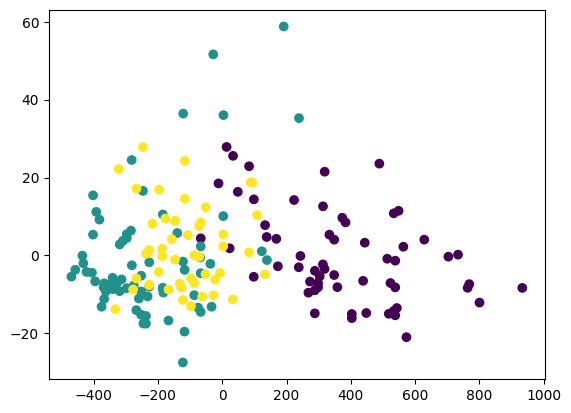
\includegraphics[width=0.8\textwidth]{output.png}
    \caption{PCA with 2 components on dataset wine}
\end{figure}


\newpage
\subsection{Exercise c)}

\begin{itemize}
    \item For K-Means: 
    \[
    s = 0.5602652844394511
    \]
    
    \item For EM-Clustering: 
    \[
    s = 0.2623333079949892
    \]
\end{itemize}

The hard assignment performed by k-means continues to be the best solution (greater silhouette).
However, the silhouette values are lower comparing with a),
what indicates that the dimensionality reduction achieved with PCA
entails an information loss that makes the clusters less distinct,
and consequently worse.
\\
\\
Furthermore, that loss indicates that the attributes with lower variance 
(filtered by PCA) are the ones that made the clusters more different 
(and with a greater silhouette).

\begin{figure}[h]
    \centering
    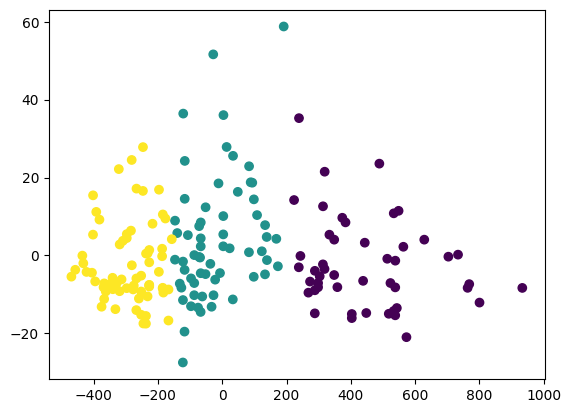
\includegraphics[width=0.8\textwidth]{output1.png}
    \caption{K-Means clustering result for the wine dataset}
\end{figure}

\begin{figure}[h!]
    \centering
    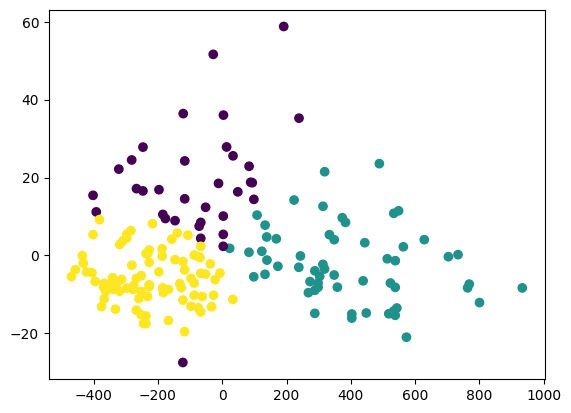
\includegraphics[width=0.8\textwidth]{output2.png}
    \caption{EM-Clustering result for the wine dataset}
\end{figure}

\clearpage

\subsection{Exercise d)}
Without PCA, k-means remains the best for this dataset too. \\
\begin{figure}[h!]
    \centering
    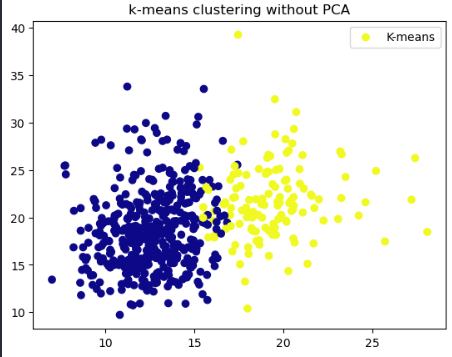
\includegraphics[width=0.8\textwidth]{04_Work4/kmeans_no-pca.png}
    \caption{shillouette = 0.6972646156059464}
\end{figure}
\begin{figure}[h!]
    \centering
    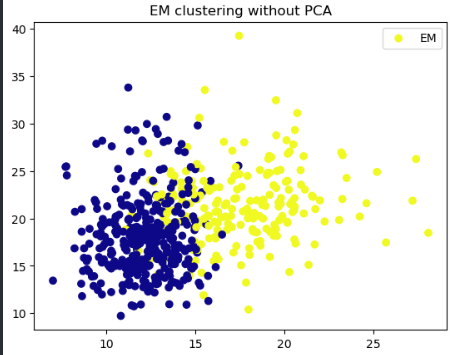
\includegraphics[width=0.8\textwidth]{04_Work4/EM_no-pca.png}
    \caption{shillouette = 0.5325475269320484}
\end{figure}

\clearpage
The same after PCA, but this time with better results.
\begin{figure}[h!]
    \centering
    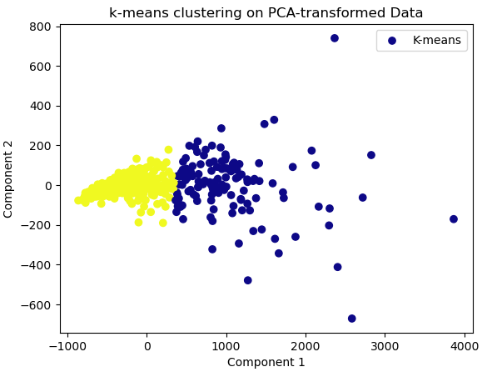
\includegraphics[width=0.8\textwidth]{04_Work4/kmeans_pca.png}
    \caption{shillouette = 0.6984195775999954}
\end{figure}
\begin{figure}[h!]
    \centering
    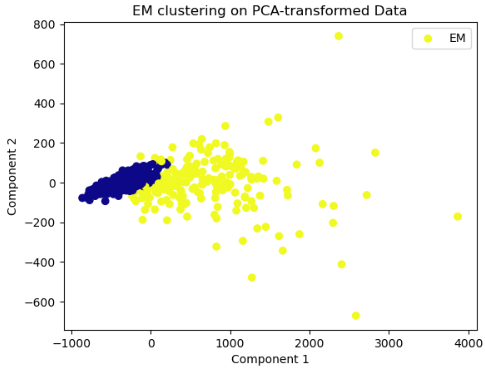
\includegraphics[width=0.8\textwidth]{04_Work4/em_pca.png}
    \caption{shillouette = 0.5865823748565955}
\end{figure}

PCA leads to better clusters (more choesive and separated, with better shillouettes)
by allowing a dimensionality reduction that specially benefits EM clustering
(more specifically its Gaussian components, making it not overfit the small amount of data after PCA). Also, the attributes that differentiate the most the clusters are the ones with higher variance.


\end{document}
